%%%%%%%%%%%%%%%%%%%%%%%%%%%%%%%%%%%%%%%%%
% Daily Laboratory Book
% LaTeX Template
%
% This template has been downloaded from:
% http://www.latextemplates.com
%
% Original author:
% Frank Kuster (http://www.ctan.org/tex-archive/macros/latex/contrib/labbook/)
%
% Important note:
% This template requires the labbook.cls file to be in the same directory as the
% .tex file. The labbook.cls file provides the necessary structure to create the
% lab book.
%
% The \lipsum[#] commands throughout this template generate dummy text
% to fill the template out. These commands should all be removed when 
% writing lab book content.
%
% HOW TO USE THIS TEMPLATE 
% Each day in the lab consists of three main things:
%
% 1. LABDAY: The first thing to put is the \labday{} command with a date in 
% curly brackets, this will make a new page and put the date in big letters 
% at the top.
%
% 2. EXPERIMENT: Next you need to specify what experiment(s) you are 
% working on with an \experiment{} command with the experiment shorthand 
% in the curly brackets. The experiment shorthand is defined in the 
% 'DEFINITION OF EXPERIMENTS' section below, this means you can 
% say \experiment{pcr} and the actual text written to the PDF will be what 
% you set the 'pcr' experiment to be. If the experiment is a one off, you can 
% just write it in the bracket without creating a shorthand. Note: if you don't 
% want to have an experiment, just leave this out and it won't be printed.
%
% 3. CONTENT: Following the experiment is the content, i.e. what progress 
% you made on the experiment that day.
%
%%%%%%%%%%%%%%%%%%%%%%%%%%%%%%%%%%%%%%%%%

%----------------------------------------------------------------------------------------
%	PACKAGES AND OTHER DOCUMENT CONFIGURATIONS
%----------------------------------------------------------------------------------------

\documentclass[idxtotoc,hyperref,openany]{labbook} % 'openany' here removes the gap page between days, erase it to restore this gap; 'oneside' can also be added to remove the shift that odd pages have to the right for easier reading

\usepackage[ 
  backref=page,
  pdfpagelabels=true,
  plainpages=false,
  colorlinks=true,
  bookmarks=true,
  pdfview=FitB]{hyperref} % Required for the hyperlinks within the PDF
  
\usepackage{booktabs} % Required for the top and bottom rules in the table
\usepackage{float} % Required for specifying the exact location of a figure or table
\usepackage{graphicx} % Required for including images
\usepackage{lipsum} % Used for inserting dummy 'Lorem ipsum' text into the template

\newcommand{\HRule}{\rule{\linewidth}{0.5mm}} % Command to make the lines in the title page
\setlength\parindent{0pt} % Removes all indentation from paragraphs

\begin{document}

%----------------------------------------------------------------------------------------
	% TITLE PAGE
%----------------------------------------------------------------------------------------

\frontmatter % Use Roman numerals for page numbers
\title{
\begin{center}
\HRule \\[0.4cm]
{\Huge \bfseries Speech Signal Processing Protokoll \\[0.5cm] \Large Master of Science}\\[0.4cm] % Degree
\HRule \\[1.5cm]
\end{center}
}
\author{\Huge Klaus-Johan Ziegert \\ \\ \LARGE
        3ziegert@informatik.uni-hamburg.de \\[2cm] 
\\ \\ \Huge John Smith \\ \\ \LARGE john@smith.com \\[2cm]} % Your name and email address
\date{Beginning 16 March 2017} % Beginning date
\mainmatter % Use Arabic numerals for page numbers

%----------------------------------------------------------------------------------------
%       DEFINITION OF EXPERIMENTS
%----------------------------------------------------------------------------------------

\newexperiment{e0101}{Fundamental frequency estimation by eye}
\newexperiment{e0102}{Block processing}
\newexperiment{e0103}{Fundamental frequency estimator}
%\newexperiment{shorthand}{Description of the experiment}
%----------------------------------------------------------------------------------------

%	LAB BOOK CONTENTS
%----------------------------------------------------------------------------------------

% Blank template to use for new days:

%\labday{Day, Date Month Year}

%\experiment{}

%Text

%-----------------------------------------

%\experiment{}

%Text

%----------------------------------------------------------------------------------------

\labday{Exercise1 : Dienstag, 17 März 2018}

\experiment{e0101}

a)

Der Befehl audioread erhält als Argument den wav-File und liefert
einen Tupel zurück:

\begin{lstlisting}
[y1,Fs1] = audioread('speech1.wav');
[y2,Fs2] = audioread('speech2.wav');
\end{lstlisting}

Die erste Rückgabe (y1 bzw. y2) ist ein Array/Liste von Samples
(Abtastwerte).  Die zweite Rückgabe (Fs2 bzw. Fs1) liefert uns
die sampling frequency (Abtastrate, auch sampling rate siehe
Exercise 2). Mit der Abtastrate kann man sowohl den Zeitpunkt
eines Samples bestimmen ( (index des Samples in y) $\backslash$
Fs) als auch die Gesamtdauer des Signals ((length(y))
$\backslash$ Fs). Die Abtastrate beider Signale ist $16000$.    

b)

Mit dem Befehl plot kann man die Signale durch die Abtastwerte y darstellen. Für die
entsprechende Zeitstellen x muss man lediglich den Index durch die
Abtastrate nehmen:

\begin{lstlisting}
	x1 = [1:length(y1)] / Fs1;
	x2 = [1:length(y2)] / Fs2;
	figure; 
	plot(x1,y1);
	figure;
	plot(x2,y2);
\end{lstlisting}

Die Plotts sind in Abbildung \ref{img:signal1} und \ref{img:signal2} zu sehen.
Um Signale besser zu vergleichen, können wir mithilfe von subplot das Anzeigefenster zurecht splitten und Teilfenster entsprechend plotten.

\begin{figure}[H]
	\centering
	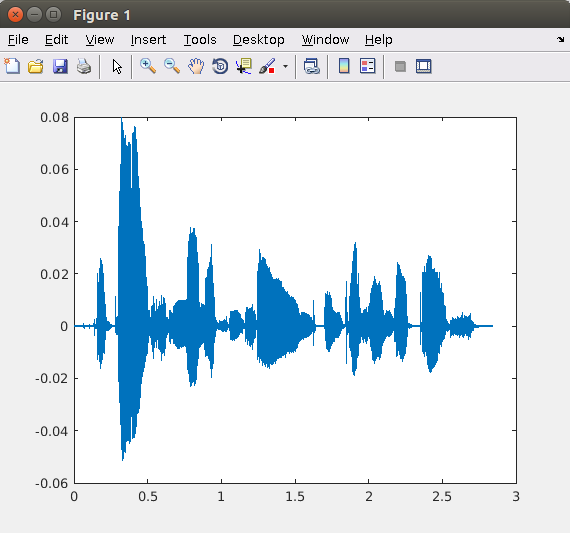
\includegraphics[width=0.6\textwidth]{./bilder/signal1.png}
	\caption{Plott des ersten Signals}
	\label{img:signal1}
\end{figure}

\begin{figure}[H]
	\centering
	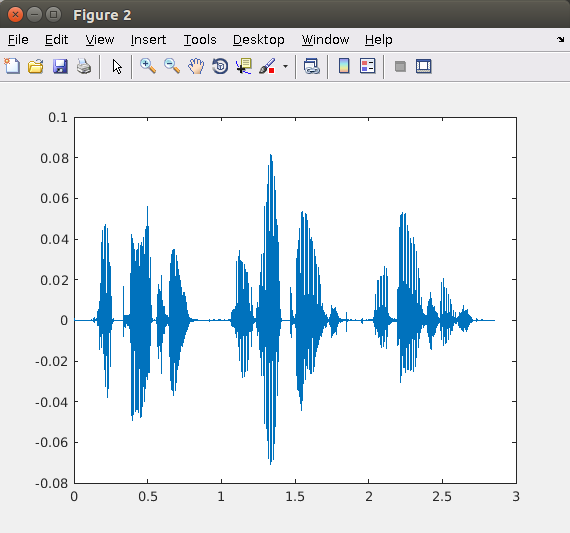
\includegraphics[width=0.6\textwidth]{./bilder/signal2.png}
	\caption{Plott des zweiten Signals}
	\label{img:signal2}
\end{figure}


Identifikation von stimmhaften etc:
\begin{itemize}
\item stimmhaft: quasi periodisch, hohe Amplituden
\item stimmlos: hat die Form von "Rauschen" 
\item silence: flach
\end{itemize}

c) 

Mithilfe von sound(lautverstärker * y(from:to),Fs) können wir den
sample-Bereich, from bis to, hören. Wenn wir der Auffassung sind, dass dieser
Bereich tatsächlich ein stimmhafter Ton ist, dann suchen wir die Grundfrequenz
wie folgt: 
\begin{itemize}
	\item Voraussetzung: Stell Zoomoption auf horizontal
	\item Zoome den entsprechenden Bereich 
	\item Zoome solange bis Wiederholungen sehbar sind
	\item Wähle eine Periode aus, messe den Abstand (Periodendauer)
	und wähle den Kehrwert als Grundfrequenz
\end{itemize}

Beispiel des zweiten deutlich erkennbaren Tons im ersten Signal:

\begin{figure}[H]
	\centering
	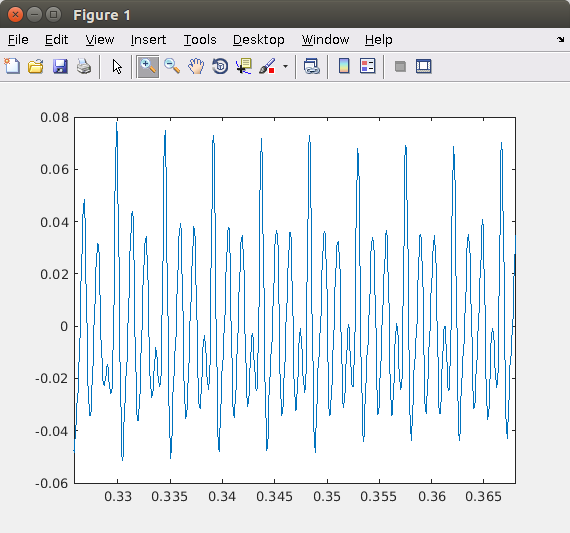
\includegraphics[width=0.6\textwidth]{./bilder/grundfrequenzsuche.png}
	\caption{Zoomen bis Wiederholung sehbar}
	\label{img:grundfrequenzsuche}
\end{figure}

\begin{figure}[H]
	\centering
	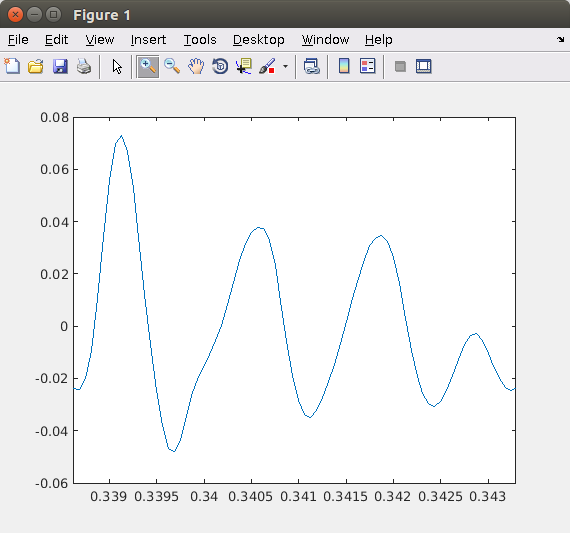
\includegraphics[width=0.6\textwidth]{./bilder/periode.png}
	\caption{Periode gezoomt}
	\label{img:periode}
\end{figure}

Die Periode beträgt aus Abbildung \ref{img:periode} geschätzt: 
$ 0.3435 s -0.3385 s = 0.005$, also einer geschätzten Grundfrequenz von $ F = 200$



% -----------------------------------------

\experiment{e0102}

Jeder Frame besteht aus einer festen Anzahl von Samples, dessen Größe durch
frame\_length in Sekunden angegeben wird.  Mit frame\_length $\cdot$ Fs erhält
man die Anzahl von Samples eines Frames. Der erste Frame fängt daher von
sekunde 0 an und endet bei Sekunde frame\_length.  Der Start des zweiten Frame wird durch
die Verschiebungen um frame\_shift nach links vom Ende des Vorgängers festgelegt.
D.h. durch die Anzahl von möglichen Verschiebung plus 1 wegen dem ersten Frame
können wir die Anzahl der benötigten Frames ermitteln:
\[
	|F| = \left \lfloor
	\frac{signal\_length - frame\_length + frame\_shift}
	{frame\_shift} \right \rfloor + 1
\]

Implementation: 
\lstinputlisting{./my_windowing.m}

% -----------------------------------------
\experiment{e0103}


% -----------------------------------------
Text


% ----------------------------------------------------------------------------------------

\end{document}
